\documentclass[a4paper, 12pt, twoside]{article}
\usepackage[utf8]{inputenc}
\usepackage[T1]{fontenc}
\usepackage[francais]{babel}
\usepackage{lmodern}
\usepackage{ae,aecompl}
\usepackage[top=2.5cm, bottom=2cm, left=3cm, right=2.5cm, headheight=15pt]{geometry}
\usepackage{graphicx}
\usepackage{eso-pic}
\usepackage{array}
\usepackage{hyperref}
\usepackage{float}

% Configuration des liens
\hypersetup{
    colorlinks=true,
    linkcolor=black,
    filecolor=magenta,      
    urlcolor=blue,
}

% Inclusion de la page de garde
\input{pagedegarde}

% --- VARIABLES DE LA PAGE DE GARDE ---
\title{Captcha sous LLM}
\entreprise{Université Paris Nanterre} 
\datedebut{7 octobre 2025}
\datefin{6 janvier 2026}

\membrea{KEBBACHE WALID - N°Etudiant : 45003317}
\membreb{YAHOU SARAH - N°Etudiant : 45011767}
\membrec{} 
\membred{}
\membree{}

\begin{document}

% --- PAGE DE GARDE ---
\pagedegarde

% --- REMERCIEMENTS ---
\section*{Remerciements}
Merci, merci à tous.

Je remercie GEMINI et ChatGPT de m'avoir grandement aidé pour le développement, qui ont agi comme de véritables \textbf{interprètes de pensée} durant ce projet.

Si l'idée originale du Dashboard sous Tkinter, l'architecture globale de \textbf{VerifBot} ainsi que \textbf{Trainmodel} viennent entièrement de nous, l'IA a été notre bras droit pour la mise en œuvre technique.

Nous lui avons \textbf{soufflé} nos concepts, nos structures et nos exigences ergonomiques, et elle s'est chargée de traduire nos idées en lignes de code fonctionnelles.

Cette collaboration nous a permis de nous concentrer sur la logique métier et la conception du système, tout en déléguant la rédaction fastidieuse du code.

Ce rapport est donc le résultat d'un travail d'équipe où l'humain a gardé la vision créative et l'IA a assuré la main-d'œuvre numérique.

\newpage

% --- TABLE DES MATIÈRES ---
\tableofcontents
\newpage

% --- INTRODUCTION ---
\section{Introduction}
Dans un web de plus en plus automatisé, la distinction entre un utilisateur humain et un robot est devenue un enjeu majeur de cybersécurité.
Ce projet, intitulé \textbf{Captcha sous LLM}, vise à concevoir une solution complète de CAPTCHA comportemental.

\begin{figure}[H]
\centering

\includegraphics[width=0.6\textwidth]{EN-Captcha-Spamschutz-12.png} 
\caption{Exemple de reCAPTCHA}
\end{figure}

Contrairement aux CAPTCHA traditionnels basés sur la lecture de texte ou la sélection d'images, notre système analyse le comportement de la souris (vitesse, accélération, hésitations, régularité des trajectoires) afin de déterminer la nature de l'utilisateur.

Le projet ne se limite pas à la détection : nous avons également développé un bot attaquant capable de \textbf{voir} l'écran et de simuler un comportement humain, afin de tester la robustesse de notre propre système.

Notre détecteur est un système hybride : un modèle de Machine Learning prend la décision principale, et en cas d'incertitude (\textbf{zone de doute}), un modèle de langage (LLM) est sollicité comme second avis afin d'améliorer la robustesse de la détection.

L'objectif final est de proposer une architecture client-serveur fonctionnelle, pilotée par un Dashboard d'administration centralisé, permettant de lancer l'ensemble sans manipulations complexes en ligne de commande.

% --- ENVIRONNEMENT DE TRAVAIL ---
\section{Environnement de travail}
Ce projet \textit{Fullstack} a nécessité la maîtrise d'un écosystème technique hétérogène, du développement web jusqu'à l'IA et l'automatisation système.

Le développement a été pensé \textit{cross-platform}, avec compatibilité Windows, macOS et Linux.

\begin{itemize}
    \item Langages : Python 3.10+ (Backend, IA, scripts), TypeScript/React (Frontend), Batch/Bash (automatisation).
    \item Outils : Git pour le versionnage, Visual Studio Code pour le développement.
    \item Architecture cible : Client (navigateur) $\leftrightarrow$ API REST (FastAPI) $\leftrightarrow$ Modèles IA (locaux \& cloud).
\end{itemize}

% --- DESCRIPTION DU PROJET ---
\section{Description du projet et objectifs}
Le projet s'articule autour de quatre piliers interconnectés, chacun jouant un rôle spécifique dans la chaîne d'acquisition--analyse--décision.

\begin{itemize}
    \item \textbf{Frontend (l'épreuve) :} application web proposant trois mini-jeux (Trace, Puzzle, Sélection d'images) conçus pour récolter des données biométriques issues des mouvements de souris.
    \item \textbf{Backend \& IA (le juge) :} API recevant les données, extrayant des caractéristiques cinématiques, puis renvoyant un verdict \textbf{Humain} ou \textbf{Robot} via un modèle de ML hybride.
    \item \textbf{Bot attaquant (l'adversaire) :} script autonome utilisant OpenCV pour repérer des éléments à l'écran et une IA générative (Gemini) pour simuler des trajectoires réalistes.
    \item \textbf{Dashboard Admin (l'orchestrateur) :} interface Tkinter permettant de lancer et gérer tous ces services sans passer par le terminal.
\end{itemize}

\subsection{Fonctionnement de la collecte}
Le navigateur collecte les points $(x,y,t)$ durant l'interaction avec les jeux, puis les envoie au backend.

Le backend normalise et transforme ces données en \textit{features} physiques (vitesse, accélération, rectitude...), et produit une prédiction via le modèle ML.

\begin{figure}[H]
\centering
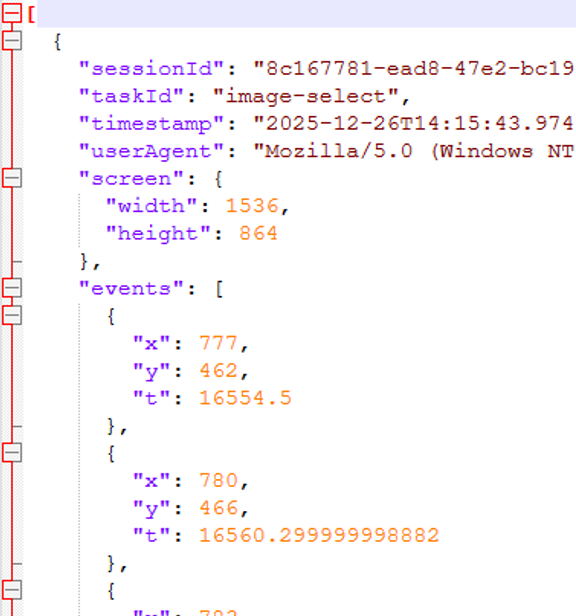
\includegraphics[width=0.8\textwidth]{json.png} 
\caption{Exemple de données collectées (JSON)}
\end{figure}

En cas d'incertitude, une logique de \textbf{zone de doute} déclenche une analyse complémentaire par Gemini afin d'améliorer la robustesse de la décision finale.

\subsection{Objectifs principaux}
\begin{itemize}
    \item Concevoir des épreuves courtes et exploitables (capables de capturer de la motricité fine).
    \item Construire une chaîne de traitement reproductible (normalisation, extraction de features, entraînement, évaluation).
    \item Démontrer la solidité du système en développant un bot attaquant réaliste.
    \item Proposer une expérience \textbf{clé en main} via un dashboard de lancement.
\end{itemize}

% --- BIBLIOTHEQUES ---
\section{Bibliothèques, Outils et technologies}
Nous avons exploité des bibliothèques spécialisées pour chaque brique du projet :

\begin{itemize}
    \item Frontend : React, TypeScript, Vite.
    \item Backend \& API : FastAPI + Uvicorn (serveur ASGI).
    \item Exposition : Ngrok (tunneling).
    \item Data science / ML : Scikit-learn (Random Forest), Pandas / NumPy, Joblib (sérialisation du modèle).
    \item Vision \& IA générative : OpenCV (cv2), Google Generative AI (Gemini).
    \item Automatisation : PyAutoGUI, subprocess, threading.
\end{itemize}

% --- TRAVAIL REALISE ---
\section{Travail réalisé}

\subsection*{A. Développement des épreuves CAPTCHA (Frontend)}
Nous avons créé trois composants React distincts afin de capturer différents aspects de la motricité :
\begin{itemize}
    \item \textbf{TraceGame} : suivi d'une ligne sinusoïdale, avec mesure de la déviation par rapport à une trajectoire attendue.
    \item \textbf{PuzzleGame} : \textit{drag \& drop} d'une pièce vers une zone cible, utile pour analyser accélération/décélération à l'approche.
    \item \textbf{ImageSelectGame} : sélection d'images (ex. chats/chiens/voitures) avec tolérance à l'erreur pour mimer le comportement humain.
\end{itemize}
Une page \textbf{Résultats} permet d'exporter les sessions (par épreuve et cumulées) et de lancer la vérification via le backend, puis d'afficher le verdict final.

Chaque mouvement de souris est enregistré sous forme de séries temporelles (X, Y, Temps) puis envoyé au serveur pour analyse.

\subsection*{B. Moteur de détection (Backend \& ML)}
Le backend implémente une chaîne de traitement complète :
\begin{itemize}
    \item \textit{Feature engineering} (\texttt{utilitis.py}) : transformation des données brutes en indicateurs physiques (vitesse moyenne, variabilité, accélération, \textit{straightness}, etc.).
    \item Modèle Random Forest (\texttt{train.py}) : entraînement sur notre dataset Humains vs Bots, avec validation croisée (Stratified K-Fold).
    \item Architecture hybride (\texttt{api.py}) : logique de doute :
    \begin{itemize}
        \item Si confiance forte, le Random Forest tranche.
        \item Si confiance intermédiaire, appel à Gemini pour une analyse contextuelle des logs et de la cohérence des patterns.
    \end{itemize}
\end{itemize}

\subsection*{C. Bot attaquant (simulation d'attaque)}
Pour éprouver notre défense, nous avons développé un bot autonome :
\begin{itemize}
    \item Vision : capture écran et détection d'éléments via filtrage HSV / traitement d'images (OpenCV) afin de repérer boutons et cibles.
    \item Trajectoires réalistes : génération d'une trajectoire (JSON) par Gemini, puis exécution avec PyAutoGUI en ajoutant des micro-pauses et imperfections.
\end{itemize}

\subsection*{D. Dashboard d'administration (Tkinter)}
Le dashboard (\texttt{APP.py}) automatise l'installation et le lancement :
\begin{itemize}
    \item Installation partielle des dépendances (librairies)
    \item Lancement parallèle (API + React) via multi-threading, garantissant une interface réactive.
\end{itemize}

% --- DIFFICULTÉS ---
\section{Difficultés rencontrées}
\begin{itemize}
    \item Normalisation : les résolutions d'écran différentes imposaient de normaliser les coordonnées entre 0.0 et 1.0 pour rendre le modèle généralisable.
    \item Latence \& asynchronisme : concilier FastAPI (async) et des appels Gemini parfois lents sans bloquer l'expérience.
    \item Vision \& scaling Windows : erreurs de clic dues au zoom/display scaling (125\%/150\%), nécessitant une récupération fiable de la résolution réelle (ctypes).
    \item Équilibre : système trop strict (faux négatifs humains) vs trop laxiste (faux positifs bots) ; la \textbf{zone de doute} + second recours Gemini a stabilisé le compromis.
\end{itemize}

Malgré leurs performances impressionnantes sur des tâches complexes, les modèles de langage (LLM) se sont révélés parfois déroutants dans un contexte de développement : ils peuvent proposer des solutions élégantes sur le papier, tout en échouant à résoudre correctement des problèmes pourtant simples ou très concrets (gestion d'un cas limite, bug de logique, incohérence de format, donner des résultats sous la bonne forme, etc...).

À plusieurs reprises, il a donc fallu revenir au code, analyser l'exécution \textbf{à la main}, comprendre l'origine exacte du dysfonctionnement et corriger directement les scripts, y compris lorsque les suggestions de Gemini étaient incomplètes ou incorrectes.

Cette difficulté nous a appris une leçon importante : un LLM est un excellent accélérateur (idées, prototypes, aide à la syntaxe), mais il ne remplace pas la compréhension du code ni la phase de débogage rigoureuse, surtout dans un projet hybride (Frontend + API + ML + automatisation).

% --- BILAN ---
\section{Bilan}

\subsection{Conclusion}
Le projet \textbf{Captcha sous LLM} constitue une réussite technique : il combine une application web, une API, un modèle de machine learning et un bot attaquant, le tout orchestré par une interface d'administration.

Nous avons réussi à :
\begin{itemize}
    \item Créer un dataset de mouvements (humains et bots).
    \item Entraîner un modèle capable de distinguer les deux avec une précision satisfaisante dans nos tests.
    \item Développer une application complète et ergonomique.
\end{itemize}

L'apport principal est la compréhension de la chaîne de la donnée : capture (React) $\rightarrow$ transformation (Python/Pandas) $\rightarrow$ apprentissage (Scikit-learn) $\rightarrow$ décision (API).

Ce travail nous a confrontés à des problématiques actuelles de cybersécurité et d'IA : un même ensemble d'outils peut servir à attaquer (bot réaliste) et à défendre (détection comportementale + modèle hybride).

Le projet nous a aussi appris à intégrer proprement des composants hétérogènes (web, ML, automatisation) dans une architecture cohérente.

\subsection{Perspectives}
\begin{itemize}
    \item Renforcement du modèle : collecter plus de données et tester un modèle séquentiel (LSTM) pour mieux exploiter la dimension temporelle.
    \item Sécurité API : ajouter une authentification (token) et des contrôles anti-rejeu.
    \item Dockerisation : conteneuriser l'ensemble pour réduire les problèmes d'installation et de compatibilité.
\end{itemize}

% --- BIBLIOGRAPHIE ---
\section{Bibliographie}
\renewcommand{\bibname}{}
\renewcommand{\refname}{}
\begin{thebibliography}{9}
\bibitem{ref1} Documentation interne du projet.
\end{thebibliography}

% --- WEBOGRAPHIE ---
\section{Webographie}
\begin{thebibliography}{9}
    \bibitem[FAS]{fastapi} FastAPI Documentation, \textbf{Run a Server Manually / Deployment}, \url{fastapi.tiangolo.com}
    \bibitem[UVI]{uvicorn} Uvicorn Documentation, \url{uvicorn.dev}
    \bibitem[SKL]{sklearn} Scikit-learn, \textbf{RandomForestClassifier — documentation}, \url{scikit-learn.org}
    \bibitem[GEM]{gemini} Google AI for Developers, \textbf{Gemini API Docs}, \url{ai.google.dev}
    \bibitem[OPC]{opencv} OpenCV Documentation, \textbf{OpenCV-Python Tutorials}, \url{docs.opencv.org}
    \bibitem[PAG]{pyautogui} PyAutoGUI Documentation, \textbf{Quickstart / Cheat Sheet}, \url{pyautogui.readthedocs.io}
\end{thebibliography}

\newpage

% --- ANNEXES ---
\section{Annexes}
\appendix
\makeatletter
\def\@seccntformat#1{Annexe~\csname the#1\endcsname:\quad}
\makeatother

% --- ANNEXE A ---
\section{Cahier des charges}

\subsection*{A.1 Contexte et démarche initiale}
Au démarrage du projet, les objectifs fonctionnels n'étaient pas encore clairement définis.
Afin de structurer le travail, nous avons d'abord réalisé une maquette de l'application web (organisation des écrans, déroulement des étapes, comportement attendu du CAPTCHA) à l'aide de ChatGPT 5 et Claude 4.5 Sonnet.

Cette maquette nous a permis de valider l'expérience utilisateur et de clarifier le fonctionnement global avant de développer.

Une fois le concept stabilisé, nous avons refait le site de zéro dans l'objectif d'obtenir une interface plus \textbf{propre}, agréable et cohérente, tout en gardant les mêmes principes d'épreuves et de collecte des données à l'aide de Gemini 3.

\subsection*{A.2 Objectifs fonctionnels}
Le site devait répondre aux besoins suivants :
\begin{itemize}
    \item Proposer un CAPTCHA comportemental composé de plusieurs épreuves (Puzzle, Trace, Image-selector).
    \item Enregistrer les sessions utilisateurs avec l'ensemble des informations nécessaires (coordonnées, temps, etc.).
    \item Permettre à l'utilisateur, à la fin d'un CAPTCHA, de télécharger ses sessions individuellement (par jeu) et également une version cumulée (\textbf{stack}) regroupant toutes les sessions en un seul fichier (par jeu).
    \item Transmettre ces données à un serveur (backend) afin qu'un programme Python puisse analyser les sessions reçues et retourner une décision.
\end{itemize}

\subsection*{A.3 Données attendues (collecte \& format)}
Chaque épreuve génère une session contenant au minimum une série temporelle de points (par exemple : $x, y, timestamp$), permettant ensuite de calculer des indicateurs cinématiques (vitesse, accélération, hésitations, rectitude).

Les sessions doivent être exportables :
\begin{itemize}
    \item Soit séparément (un fichier par épreuve).
    \item Soit regroupées (un fichier unique cumulant toutes les épreuves).
\end{itemize}

\subsection*{A.4 Constitution du jeu de données (phase de validation)}
Pour valider rapidement la faisabilité, nous avons constitué un premier dataset minimal :
\begin{itemize}
    \item 120 sessions humaines.
    \item 100 sessions générées par un bot LLM-VL.
\end{itemize}
Ce jeu initial avait pour objectif principal de vérifier que la chaîne \textbf{collecte $\rightarrow$ extraction $\rightarrow$ classification} fonctionne techniquement avant d'augmenter le volume de données.

\subsection*{A.5 Adversaire : Bot VL (vision + mouvements humains)}
Le cahier des charges incluait volontairement un \textbf{attaquant} afin d'évaluer la robustesse du système. Ce bot devait :
\begin{itemize}
    \item Prendre une capture d'écran.
    \item Utiliser OpenCV pour détecter l'épreuve/captcha à résoudre (repérage des zones et éléments de l'interface).
    \item Résoudre l'épreuve, puis demander à Gemini de générer/adapter une trajectoire de souris plus \textbf{humaine} (courbes, imperfections, micro-pauses), et exécuter ces mouvements OU demander à Gemini les réponses adéquates pour résoudre le captcha.
\end{itemize}

Plus précisément :
\begin{itemize}
    \item Pour le \textbf{puzzle} : mettre le cube dans la bonne case, demander à Gemini de rendre les mouvements humains !
    \item Pour l'épreuve \textbf{image-selector} : utiliser Gemini et OpenCV pour identifier les bonnes images à sélectionner, puis cliquer en conservant un mouvement réaliste.
    \item Pour l'épreuve \textbf{Trace} : suivre une ligne en produisant des mouvements humains, non parfaitement rectilignes.
\end{itemize}

\subsection*{A.6 Backend et communication}
Un backend devait être mis en place pour recevoir les fichiers de sessions envoyés par le client.
L'objectif est que l'analyse s'effectue sur un ordinateur serveur exécutant un programme Python dédié.

\subsection*{A.7 Détection : modèle ML + arbitrage LLM (CAPTCHA intelligent)}
La détection repose sur un modèle de Machine Learning entraîné en Python (Scikit-learn). L'organisation logicielle attendue est la suivante :
\begin{itemize}
    \item Un script \textbf{utilitis} regroupant les commandes/fonctions clés (pré-traitement, extraction de features).
    \item Un script d'entraînement \textbf{train} produisant un modèle sérialisé (fichiers \texttt{.pkl}).
    \item Un script \textbf{api} chargé d'utiliser le modèle entraîné pour effectuer les prédictions.
\end{itemize}
Exposition de l'API via FastAPI et exécution via Uvicorn.

Fonctionnement de la décision :
\begin{enumerate}
    \item L'API charge le modèle entraîné (\texttt{.pkl}).
    \item Elle analyse les coordonnées reçues et renvoie une probabilité entre 0 et 1.
    \item Plus la valeur est élevée, plus le comportement est considéré \textbf{bot} (et inversement, plus c'est faible, plus c'est \textbf{humain}).
    \item Zone de doute : si la probabilité est entre 30\% et 80\%, le système déclenche un second avis via Gemini (LLM) ; c'est ce dernier qui tranche la décision finale.
\end{enumerate}

\subsection*{A.8 Hors périmètre (ce que le système ne doit pas faire)}
\begin{itemize}
    \item Le système ne doit pas exiger de CAPTCHA \textbf{classiques} (texte déformé illisible, audio, etc.) : la détection doit rester principalement comportementale (mouvements de souris).
    \item Le système ne doit pas bloquer l'utilisateur sans explication : il doit toujours renvoyer un verdict explicite (\textbf{Humain} / \textbf{Robot}) accompagné d'un score/indice de confiance.
    \item Le backend ne doit pas dépendre uniquement du LLM : le modèle local (Random Forest) doit rester la première décision, et le LLM ne doit intervenir qu'en \textbf{zone de doute}.
    \item L'application ne doit pas nécessiter une configuration manuelle complexe pour être testée (objectif \textbf{lancement simple} via l'orchestrateur / scripts).
    \item Le système ne doit pas collecter des données personnelles directes (nom, email, etc.) : seules les données nécessaires à l'analyse de session (événements de souris et métriques) doivent être utilisées (RGPD).
    \item Le bot attaquant ne doit pas servir à des usages malveillants hors cadre du projet : il est uniquement un outil de test interne pour évaluer la robustesse du CAPTCHA.
\end{itemize}

% --- ANNEXE B ---
\section{Exemple d'exécution du projet}

L'utilisateur lance l'application (Dashboard / lancement des services).

\begin{figure}[H]
\centering
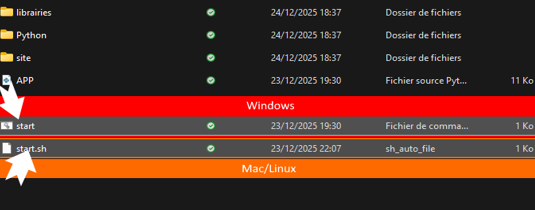
\includegraphics[width=0.4\textwidth]{ANNEXEEB_Explication1.png} 
\end{figure}

\begin{figure}[H]
\centering
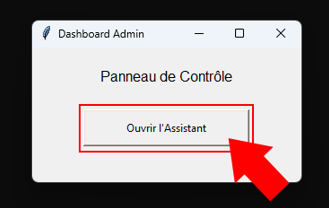
\includegraphics[width=0.6\textwidth]{ANNEXEEB_Explication2.png} 
\end{figure}
\begin{figure}[H]
\centering
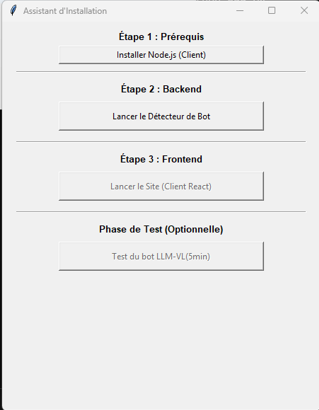
\includegraphics[width=0.6\textwidth]{ANNEXEEB_Explication3.png} 
\end{figure}

L'utilisateur ouvre l'interface web et démarre le CAPTCHA.
L'utilisateur réalise les 3 épreuves : Puzzle, Sélection d'images, Trace.

\begin{figure}[H]
\centering
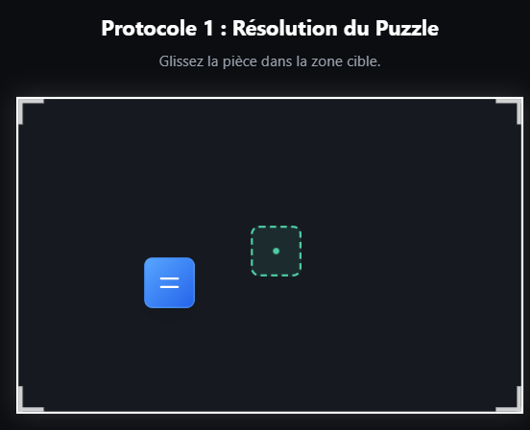
\includegraphics[width=0.3\textwidth]{ANNEXEEB_Explication4.png}
\hfill
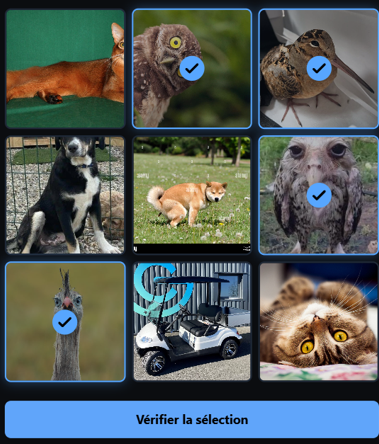
\includegraphics[width=0.3\textwidth]{ANNEXEEB_Explication5.png}
\hfill
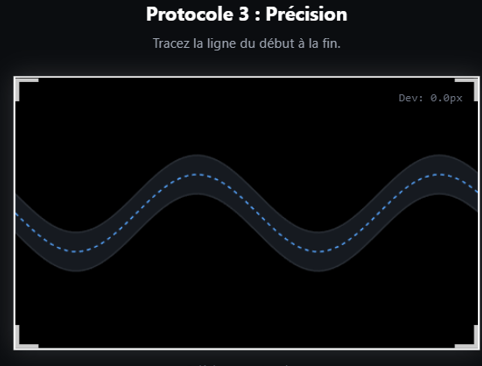
\includegraphics[width=0.3\textwidth]{ANNEXEEB_Explication6.png}
\caption{Les épreuves}
\end{figure}

À la fin, une page \textbf{Résultats} s'affiche : elle résume la réussite des épreuves et affiche des indicateurs simples sur le mouvement envoyé à l'adresse \texttt{localhost:8000/analyze/\$\{notre jeu\}} qui va être reçu par notre \texttt{api.py}.

\begin{figure}[H]
\centering
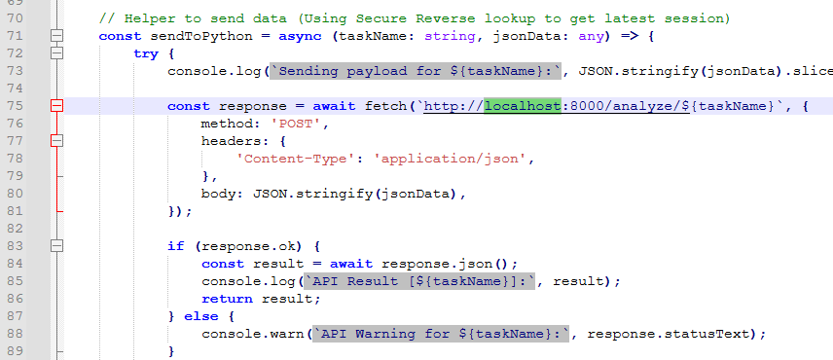
\includegraphics[width=0.8\textwidth]{ANNEXEEB_Explication7.png} 
\end{figure}

L'utilisateur peut télécharger les fichiers de session (par épreuve) ainsi qu'un export d'historique pour l'entraînement/les tests.

\begin{figure}[H]
\centering
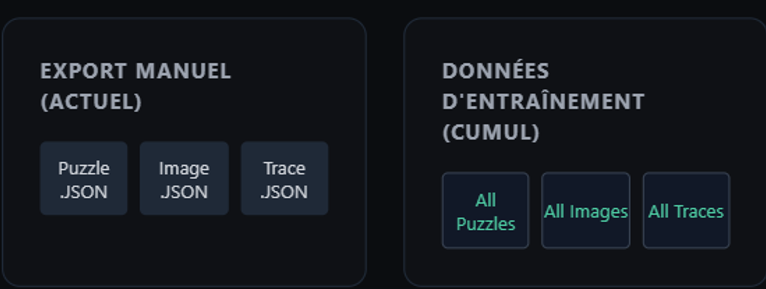
\includegraphics[width=0.8\textwidth]{ANNEXEEB_Explication8.png} 
\end{figure}

L'utilisateur clique sur \textbf{Lancer la vérification} : les données sont envoyées au backend, puis un verdict final \textbf{Humain / Robot} est affiché avec un score de confiance.

\begin{figure}[H]
\centering

\includegraphics[width=0.6\textwidth]{ANNEXEEB_Explication9.png} 
\end{figure}

En cas d'incertitude, le système effectue une vérification renforcée (CAPTCHA intelligent : second avis par LLM) avant de trancher.

\begin{figure}[H]
\centering
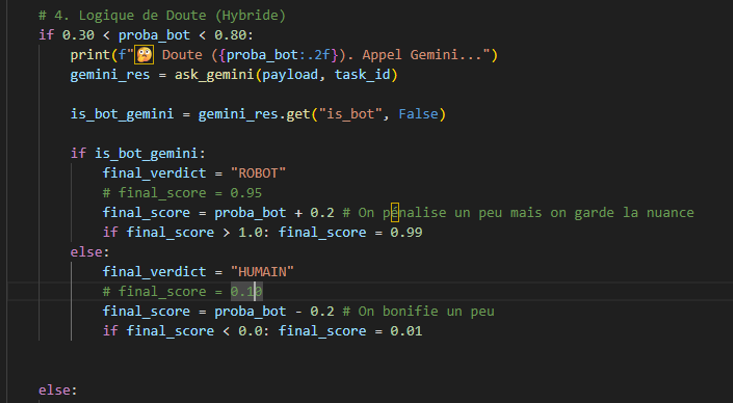
\includegraphics[width=0.8\textwidth]{ANNEXEEB_Explication10.png} 
\end{figure}

% --- ANNEXE C ---
\section{Manuel d'utilisation}

\subsection*{Prérequis}
\begin{itemize}
    \item Le projet est compatible Windows (de préférence) / macOS / Linux (scripts \texttt{.bat} pour Windows et \texttt{.sh} pour macOS/Linux).
    \item Installer Python 3.10+ (Python 3.14 est à éviter).
    \item Installer Node.js (nécessaire au Frontend React) !
    \item Réseau : ports ouverts en local ET LIBRES ! (8000 pour l'API et 3000 pour le Frontend).
    \item Une clé API Gemini si l'analyse \textbf{second avis} est activée (en cas de \textbf{zone de doute}, la réponse peut être plus lente car un appel externe est effectué).
\end{itemize}

Avant de lancer un test, vérifier que le site est accessible à l'URL locale (ex : \url{http://localhost:3000}).

\begin{figure}[H]
\centering
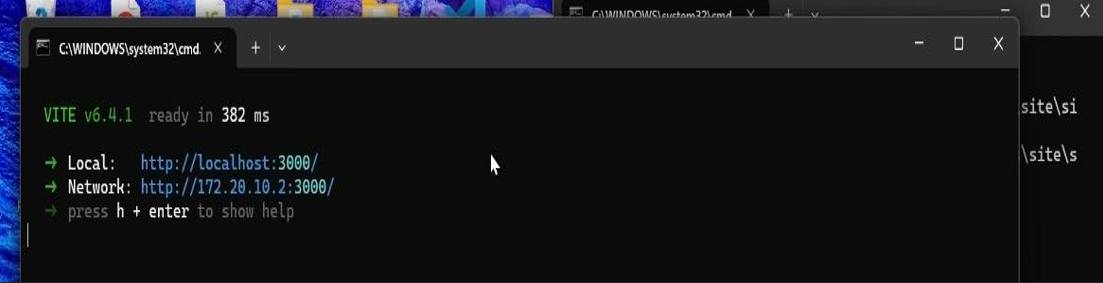
\includegraphics[width=0.8\textwidth]{ANNEXEEB_Explication11.png} 
\end{figure}

\subsection*{Installation (première exécution)}
Se placer à la racine du projet.
Installer toutes les dépendances :
\begin{itemize}
    \item Backend : installation des dépendances Python (incluant FastAPI et Uvicorn, qui ont causé des erreurs lorsqu'ils n'étaient pas présents dans la liste des dépendances).
    \item Placer la clé Gemini dans les scripts suivants : \texttt{LLM-VL-1.py}, \texttt{LLM-VL-2.py} dans \texttt{/site/Python/Trainmodel}.
\end{itemize}

\begin{figure}[H]
\centering
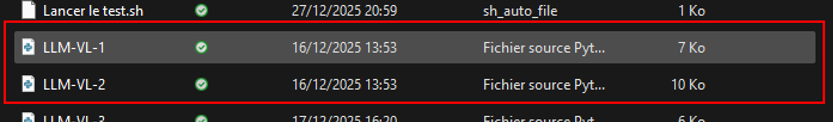
\includegraphics[width=0.8\textwidth]{ANNEXEEB_Explication12.png} 
\end{figure}
\begin{figure}[H]
\centering
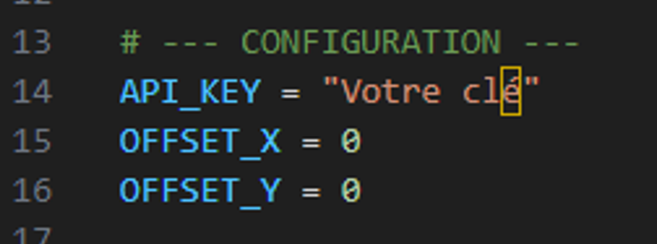
\includegraphics[width=0.8\textwidth]{ANNEXEEB_Explication13.png} 
\end{figure}

\begin{itemize}
    \item Ainsi que \texttt{API.py} dans \texttt{/site/Python/Verifbot/src}.
\end{itemize}



\begin{figure}[H]
\centering
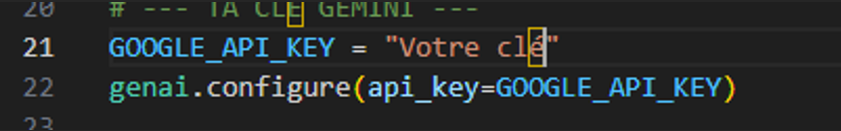
\includegraphics[width=0.6\textwidth]{ANNEXEEB_Explication14.png} 
\end{figure}

\subsection*{Lancement via Dashboard (recommandé)}
\begin{enumerate}
    \item Lancer le Dashboard : exécuter \texttt{start.bat} (ou exécuter \texttt{start.sh} sous macOS/Linux).
    \item Si le \texttt{start.bat} ou \texttt{start.sh} ne fonctionne pas, ouvrez \texttt{APP.py} (\texttt{python APP.py} dans le CMD).
    \item Cliquer sur \textbf{Ouvrir l'Assistant}.
    \item (Si nécessaire) cliquer sur \textbf{Installer Node.js (Client)}.
    \item Cliquer sur \textbf{Lancer le Détecteur de Bot} (Backend API).
    \item Cliquer sur \textbf{Lancer le Site (Client React)} (Frontend).
\end{enumerate}

\begin{figure}[H]
\centering
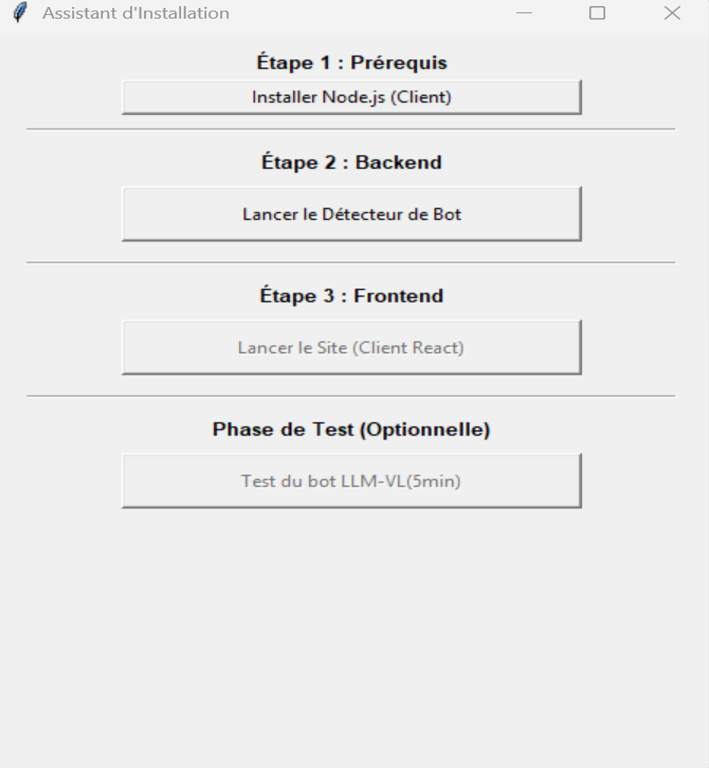
\includegraphics[width=0.5\textwidth]{ANNEXEEB_Explication15.png} 
\end{figure}

Votre site est maintenant accessible (ça peut prendre du temps en fonction de la puissance du PC) au lien suivant : \url{http://localhost:3000}.

\subsection*{Optionnel : test automatique du bot (LLM-VL)}
Cliquer sur le bouton \textbf{Test du bot LLM-VL (5 min)} (bouton bleu).

\begin{figure}[H]
\centering
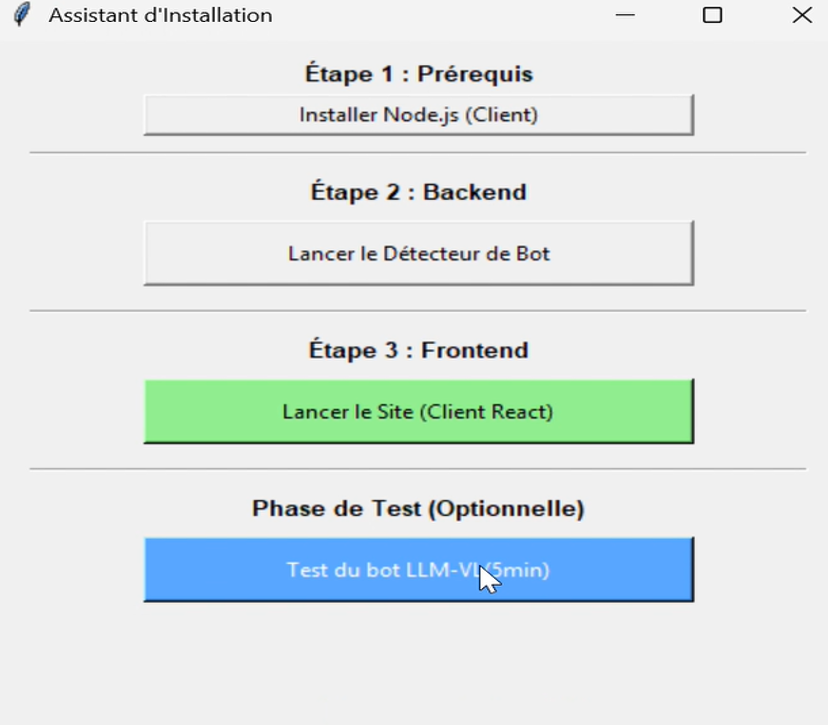
\includegraphics[width=0.5\textwidth]{ANNEXEEB_Explication16.png}
\end{figure}


Le système ouvre le navigateur, le passe en plein écran, clique sur \textbf{Initialiser}, puis exécute successivement \texttt{LLM-VL-1.py}, \texttt{LLM-VL-2.py}, \texttt{LLM-VL-3.py}.
Ne touchez à rien et laissez la magie s'opérer.

Comportement selon le système :
\begin{itemize}
    \item Windows : exécution via scripts \texttt{.bat} (ouverture d'un terminal \texttt{cmd}).
    \item macOS / Linux : exécution via scripts \texttt{.sh}, avec tentative automatique de rendu exécutable (équivalent à \texttt{chmod +x}, requis sur macOS/Linux pour lancer un script).
\end{itemize}

\subsection*{Lancement manuel (si besoin, sans Dashboard)}
Cette méthode sert de plan B en cas de blocage du Dashboard.

\textbf{Lancement du Site :}
Lancer le site : pour cela localisez l'emplacement du site (\texttt{site/site}), tapez \textbf{cmd} dans la barre d'adresse.

\begin{figure}[H]
\centering
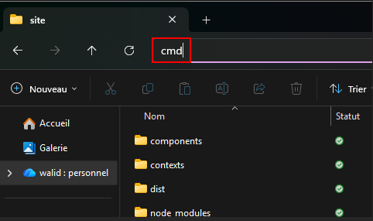
\includegraphics[width=0.6\textwidth]{ANNEXEEB_Explication17.png}
\end{figure}

Ou lancer le CMD/Terminal et accéder au dossier où le site se situe en utilisant \texttt{cd}.
\begin{figure}[H]
\centering
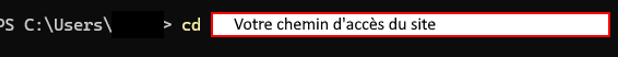
\includegraphics[width=0.8\textwidth]{ANNEXEEB_Explication18.png}
\end{figure}

Puis exécutez les commandes suivantes :
\begin{itemize}
    \item \texttt{npm install}
    \item \texttt{npm run build}
    \item \texttt{npm run dev}
\end{itemize}
Votre site est maintenant accessible au lien suivant : \url{http://localhost:3000}.

\textbf{Lancement de l'API détecteur de bot :}
Backend : lancer l'API, \texttt{/site/Python/Verifbot/src/Api.py} avec Uvicorn.
Vérification : accéder ensuite à la documentation interactive FastAPI via \texttt{/docs} (ex. \url{http://localhost:8000/docs}).

\subsection*{Utilisation (passage du CAPTCHA)}
\begin{enumerate}
    \item Ouvrir le site (lien local) et cliquer sur le bouton d'initialisation/démarrage du test.
    \item Réaliser les épreuves (tracé, puzzle, sélection d'images) de manière naturelle.
    \item Le backend renvoie un verdict Humain ou Robot ; en cas de doute, une vérification supplémentaire via Gemini peut être déclenchée (temps de réponse plus long).
\end{enumerate}

Optionnel : vous pouvez lancer un test par LLM en cliquant sur \textbf{Lancer le test.cmd} (ou \textbf{Lancer le test.sh} sur Linux/mac) dans \texttt{/site/Python/Trainmodel}.

\begin{figure}[H]
\centering
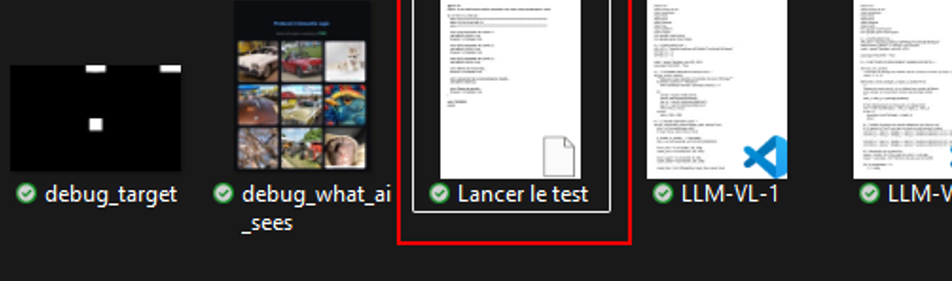
\includegraphics[width=0.8\textwidth]{ANNEXEEB_Explication19.png}
\end{figure}

Accédez au site et cliquez sur \textbf{Initialiser le protocole} et laissez la magie s'opérer.
Ou ouvrez manuellement :
\begin{itemize}
    \item \texttt{LLM-VL-1.py} pour le puzzle, donc le protocole 1.
    \item \texttt{LLM-VL-2.py} pour le protocole 2.
    \item \texttt{LLM-VL-3.py} pour le protocole 3.
\end{itemize}

\textit{Point important : mettre la fenêtre en plein écran et initialiser le protocole avant de lancer certains tests (sinon la détection/automatisation peut être perturbée et confondre par des icônes aux alentours).}

\end{document}
